
% Default to the notebook output style

    


% Inherit from the specified cell style.




    
\documentclass[11pt]{article}

    
    
    \usepackage[T1]{fontenc}
    % Nicer default font (+ math font) than Computer Modern for most use cases
    \usepackage{mathpazo}

    % Basic figure setup, for now with no caption control since it's done
    % automatically by Pandoc (which extracts ![](path) syntax from Markdown).
    \usepackage{graphicx}
    \usepackage{float}
    % We will generate all images so they have a width \maxwidth. This means
    % that they will get their normal width if they fit onto the page, but
    % are scaled down if they would overflow the margins.
    \makeatletter
    \def\maxwidth{\ifdim\Gin@nat@width>\linewidth\linewidth
    \else\Gin@nat@width\fi}
    \makeatother
    \let\Oldincludegraphics\includegraphics
    % Set max figure width to be 80% of text width, for now hardcoded.
    \renewcommand{\includegraphics}[1]{\Oldincludegraphics[width=.8\maxwidth]{#1}}
    % Ensure that by default, figures have no caption (until we provide a
    % proper Figure object with a Caption API and a way to capture that
    % in the conversion process - todo).
    \usepackage{caption}
    \DeclareCaptionLabelFormat{nolabel}{}
    \captionsetup{labelformat=nolabel}

    \usepackage{adjustbox} % Used to constrain images to a maximum size 
    \usepackage{xcolor} % Allow colors to be defined
    \usepackage{enumerate} % Needed for markdown enumerations to work
    \usepackage{geometry} % Used to adjust the document margins
    \usepackage{amsmath} % Equations
    \usepackage{amssymb} % Equations
    \usepackage{textcomp} % defines textquotesingle
    % Hack from http://tex.stackexchange.com/a/47451/13684:
    \AtBeginDocument{%
        \def\PYZsq{\textquotesingle}% Upright quotes in Pygmentized code
    }
    \usepackage{upquote} % Upright quotes for verbatim code
    \usepackage{eurosym} % defines \euro
    \usepackage[mathletters]{ucs} % Extended unicode (utf-8) support
    \usepackage[utf8x]{inputenc} % Allow utf-8 characters in the tex document
    \usepackage{fancyvrb} % verbatim replacement that allows latex
    \usepackage{grffile} % extends the file name processing of package graphics 
                         % to support a larger range 
    % The hyperref package gives us a pdf with properly built
    % internal navigation ('pdf bookmarks' for the table of contents,
    % internal cross-reference links, web links for URLs, etc.)
    \usepackage{hyperref}
    \usepackage{longtable} % longtable support required by pandoc >1.10
    \usepackage{booktabs}  % table support for pandoc > 1.12.2
    \usepackage[inline]{enumitem} % IRkernel/repr support (it uses the enumerate* environment)
    \usepackage[normalem]{ulem} % ulem is needed to support strikethroughs (\sout)
                                % normalem makes italics be italics, not underlines
    \usepackage{mathrsfs}
    

    
    
    % Colors for the hyperref package
    \definecolor{urlcolor}{rgb}{0,.145,.698}
    \definecolor{linkcolor}{rgb}{.71,0.21,0.01}
    \definecolor{citecolor}{rgb}{.12,.54,.11}

    % ANSI colors
    \definecolor{ansi-black}{HTML}{3E424D}
    \definecolor{ansi-black-intense}{HTML}{282C36}
    \definecolor{ansi-red}{HTML}{E75C58}
    \definecolor{ansi-red-intense}{HTML}{B22B31}
    \definecolor{ansi-green}{HTML}{00A250}
    \definecolor{ansi-green-intense}{HTML}{007427}
    \definecolor{ansi-yellow}{HTML}{DDB62B}
    \definecolor{ansi-yellow-intense}{HTML}{B27D12}
    \definecolor{ansi-blue}{HTML}{208FFB}
    \definecolor{ansi-blue-intense}{HTML}{0065CA}
    \definecolor{ansi-magenta}{HTML}{D160C4}
    \definecolor{ansi-magenta-intense}{HTML}{A03196}
    \definecolor{ansi-cyan}{HTML}{60C6C8}
    \definecolor{ansi-cyan-intense}{HTML}{258F8F}
    \definecolor{ansi-white}{HTML}{C5C1B4}
    \definecolor{ansi-white-intense}{HTML}{A1A6B2}
    \definecolor{ansi-default-inverse-fg}{HTML}{FFFFFF}
    \definecolor{ansi-default-inverse-bg}{HTML}{000000}

    % commands and environments needed by pandoc snippets
    % extracted from the output of `pandoc -s`
    \providecommand{\tightlist}{%
      \setlength{\itemsep}{0pt}\setlength{\parskip}{0pt}}
    \DefineVerbatimEnvironment{Highlighting}{Verbatim}{commandchars=\\\{\}}
    % Add ',fontsize=\small' for more characters per line
    \newenvironment{Shaded}{}{}
    \newcommand{\KeywordTok}[1]{\textcolor[rgb]{0.00,0.44,0.13}{\textbf{{#1}}}}
    \newcommand{\DataTypeTok}[1]{\textcolor[rgb]{0.56,0.13,0.00}{{#1}}}
    \newcommand{\DecValTok}[1]{\textcolor[rgb]{0.25,0.63,0.44}{{#1}}}
    \newcommand{\BaseNTok}[1]{\textcolor[rgb]{0.25,0.63,0.44}{{#1}}}
    \newcommand{\FloatTok}[1]{\textcolor[rgb]{0.25,0.63,0.44}{{#1}}}
    \newcommand{\CharTok}[1]{\textcolor[rgb]{0.25,0.44,0.63}{{#1}}}
    \newcommand{\StringTok}[1]{\textcolor[rgb]{0.25,0.44,0.63}{{#1}}}
    \newcommand{\CommentTok}[1]{\textcolor[rgb]{0.38,0.63,0.69}{\textit{{#1}}}}
    \newcommand{\OtherTok}[1]{\textcolor[rgb]{0.00,0.44,0.13}{{#1}}}
    \newcommand{\AlertTok}[1]{\textcolor[rgb]{1.00,0.00,0.00}{\textbf{{#1}}}}
    \newcommand{\FunctionTok}[1]{\textcolor[rgb]{0.02,0.16,0.49}{{#1}}}
    \newcommand{\RegionMarkerTok}[1]{{#1}}
    \newcommand{\ErrorTok}[1]{\textcolor[rgb]{1.00,0.00,0.00}{\textbf{{#1}}}}
    \newcommand{\NormalTok}[1]{{#1}}
    
    % Additional commands for more recent versions of Pandoc
    \newcommand{\ConstantTok}[1]{\textcolor[rgb]{0.53,0.00,0.00}{{#1}}}
    \newcommand{\SpecialCharTok}[1]{\textcolor[rgb]{0.25,0.44,0.63}{{#1}}}
    \newcommand{\VerbatimStringTok}[1]{\textcolor[rgb]{0.25,0.44,0.63}{{#1}}}
    \newcommand{\SpecialStringTok}[1]{\textcolor[rgb]{0.73,0.40,0.53}{{#1}}}
    \newcommand{\ImportTok}[1]{{#1}}
    \newcommand{\DocumentationTok}[1]{\textcolor[rgb]{0.73,0.13,0.13}{\textit{{#1}}}}
    \newcommand{\AnnotationTok}[1]{\textcolor[rgb]{0.38,0.63,0.69}{\textbf{\textit{{#1}}}}}
    \newcommand{\CommentVarTok}[1]{\textcolor[rgb]{0.38,0.63,0.69}{\textbf{\textit{{#1}}}}}
    \newcommand{\VariableTok}[1]{\textcolor[rgb]{0.10,0.09,0.49}{{#1}}}
    \newcommand{\ControlFlowTok}[1]{\textcolor[rgb]{0.00,0.44,0.13}{\textbf{{#1}}}}
    \newcommand{\OperatorTok}[1]{\textcolor[rgb]{0.40,0.40,0.40}{{#1}}}
    \newcommand{\BuiltInTok}[1]{{#1}}
    \newcommand{\ExtensionTok}[1]{{#1}}
    \newcommand{\PreprocessorTok}[1]{\textcolor[rgb]{0.74,0.48,0.00}{{#1}}}
    \newcommand{\AttributeTok}[1]{\textcolor[rgb]{0.49,0.56,0.16}{{#1}}}
    \newcommand{\InformationTok}[1]{\textcolor[rgb]{0.38,0.63,0.69}{\textbf{\textit{{#1}}}}}
    \newcommand{\WarningTok}[1]{\textcolor[rgb]{0.38,0.63,0.69}{\textbf{\textit{{#1}}}}}
    
    
    % Define a nice break command that doesn't care if a line doesn't already
    % exist.
    \def\br{\hspace*{\fill} \\* }
    % Math Jax compatibility definitions
    \def\gt{>}
    \def\lt{<}
    \let\Oldtex\TeX
    \let\Oldlatex\LaTeX
    \renewcommand{\TeX}{\textrm{\Oldtex}}
    \renewcommand{\LaTeX}{\textrm{\Oldlatex}}
    % Document parameters
    % Document title
    \title{Assignment 10}
    
    
    \author{Jiarong Ye}
    
    

    % Pygments definitions
    
\makeatletter
\def\PY@reset{\let\PY@it=\relax \let\PY@bf=\relax%
    \let\PY@ul=\relax \let\PY@tc=\relax%
    \let\PY@bc=\relax \let\PY@ff=\relax}
\def\PY@tok#1{\csname PY@tok@#1\endcsname}
\def\PY@toks#1+{\ifx\relax#1\empty\else%
    \PY@tok{#1}\expandafter\PY@toks\fi}
\def\PY@do#1{\PY@bc{\PY@tc{\PY@ul{%
    \PY@it{\PY@bf{\PY@ff{#1}}}}}}}
\def\PY#1#2{\PY@reset\PY@toks#1+\relax+\PY@do{#2}}

\expandafter\def\csname PY@tok@w\endcsname{\def\PY@tc##1{\textcolor[rgb]{0.73,0.73,0.73}{##1}}}
\expandafter\def\csname PY@tok@c\endcsname{\let\PY@it=\textit\def\PY@tc##1{\textcolor[rgb]{0.25,0.50,0.50}{##1}}}
\expandafter\def\csname PY@tok@cp\endcsname{\def\PY@tc##1{\textcolor[rgb]{0.74,0.48,0.00}{##1}}}
\expandafter\def\csname PY@tok@k\endcsname{\let\PY@bf=\textbf\def\PY@tc##1{\textcolor[rgb]{0.00,0.50,0.00}{##1}}}
\expandafter\def\csname PY@tok@kp\endcsname{\def\PY@tc##1{\textcolor[rgb]{0.00,0.50,0.00}{##1}}}
\expandafter\def\csname PY@tok@kt\endcsname{\def\PY@tc##1{\textcolor[rgb]{0.69,0.00,0.25}{##1}}}
\expandafter\def\csname PY@tok@o\endcsname{\def\PY@tc##1{\textcolor[rgb]{0.40,0.40,0.40}{##1}}}
\expandafter\def\csname PY@tok@ow\endcsname{\let\PY@bf=\textbf\def\PY@tc##1{\textcolor[rgb]{0.67,0.13,1.00}{##1}}}
\expandafter\def\csname PY@tok@nb\endcsname{\def\PY@tc##1{\textcolor[rgb]{0.00,0.50,0.00}{##1}}}
\expandafter\def\csname PY@tok@nf\endcsname{\def\PY@tc##1{\textcolor[rgb]{0.00,0.00,1.00}{##1}}}
\expandafter\def\csname PY@tok@nc\endcsname{\let\PY@bf=\textbf\def\PY@tc##1{\textcolor[rgb]{0.00,0.00,1.00}{##1}}}
\expandafter\def\csname PY@tok@nn\endcsname{\let\PY@bf=\textbf\def\PY@tc##1{\textcolor[rgb]{0.00,0.00,1.00}{##1}}}
\expandafter\def\csname PY@tok@ne\endcsname{\let\PY@bf=\textbf\def\PY@tc##1{\textcolor[rgb]{0.82,0.25,0.23}{##1}}}
\expandafter\def\csname PY@tok@nv\endcsname{\def\PY@tc##1{\textcolor[rgb]{0.10,0.09,0.49}{##1}}}
\expandafter\def\csname PY@tok@no\endcsname{\def\PY@tc##1{\textcolor[rgb]{0.53,0.00,0.00}{##1}}}
\expandafter\def\csname PY@tok@nl\endcsname{\def\PY@tc##1{\textcolor[rgb]{0.63,0.63,0.00}{##1}}}
\expandafter\def\csname PY@tok@ni\endcsname{\let\PY@bf=\textbf\def\PY@tc##1{\textcolor[rgb]{0.60,0.60,0.60}{##1}}}
\expandafter\def\csname PY@tok@na\endcsname{\def\PY@tc##1{\textcolor[rgb]{0.49,0.56,0.16}{##1}}}
\expandafter\def\csname PY@tok@nt\endcsname{\let\PY@bf=\textbf\def\PY@tc##1{\textcolor[rgb]{0.00,0.50,0.00}{##1}}}
\expandafter\def\csname PY@tok@nd\endcsname{\def\PY@tc##1{\textcolor[rgb]{0.67,0.13,1.00}{##1}}}
\expandafter\def\csname PY@tok@s\endcsname{\def\PY@tc##1{\textcolor[rgb]{0.73,0.13,0.13}{##1}}}
\expandafter\def\csname PY@tok@sd\endcsname{\let\PY@it=\textit\def\PY@tc##1{\textcolor[rgb]{0.73,0.13,0.13}{##1}}}
\expandafter\def\csname PY@tok@si\endcsname{\let\PY@bf=\textbf\def\PY@tc##1{\textcolor[rgb]{0.73,0.40,0.53}{##1}}}
\expandafter\def\csname PY@tok@se\endcsname{\let\PY@bf=\textbf\def\PY@tc##1{\textcolor[rgb]{0.73,0.40,0.13}{##1}}}
\expandafter\def\csname PY@tok@sr\endcsname{\def\PY@tc##1{\textcolor[rgb]{0.73,0.40,0.53}{##1}}}
\expandafter\def\csname PY@tok@ss\endcsname{\def\PY@tc##1{\textcolor[rgb]{0.10,0.09,0.49}{##1}}}
\expandafter\def\csname PY@tok@sx\endcsname{\def\PY@tc##1{\textcolor[rgb]{0.00,0.50,0.00}{##1}}}
\expandafter\def\csname PY@tok@m\endcsname{\def\PY@tc##1{\textcolor[rgb]{0.40,0.40,0.40}{##1}}}
\expandafter\def\csname PY@tok@gh\endcsname{\let\PY@bf=\textbf\def\PY@tc##1{\textcolor[rgb]{0.00,0.00,0.50}{##1}}}
\expandafter\def\csname PY@tok@gu\endcsname{\let\PY@bf=\textbf\def\PY@tc##1{\textcolor[rgb]{0.50,0.00,0.50}{##1}}}
\expandafter\def\csname PY@tok@gd\endcsname{\def\PY@tc##1{\textcolor[rgb]{0.63,0.00,0.00}{##1}}}
\expandafter\def\csname PY@tok@gi\endcsname{\def\PY@tc##1{\textcolor[rgb]{0.00,0.63,0.00}{##1}}}
\expandafter\def\csname PY@tok@gr\endcsname{\def\PY@tc##1{\textcolor[rgb]{1.00,0.00,0.00}{##1}}}
\expandafter\def\csname PY@tok@ge\endcsname{\let\PY@it=\textit}
\expandafter\def\csname PY@tok@gs\endcsname{\let\PY@bf=\textbf}
\expandafter\def\csname PY@tok@gp\endcsname{\let\PY@bf=\textbf\def\PY@tc##1{\textcolor[rgb]{0.00,0.00,0.50}{##1}}}
\expandafter\def\csname PY@tok@go\endcsname{\def\PY@tc##1{\textcolor[rgb]{0.53,0.53,0.53}{##1}}}
\expandafter\def\csname PY@tok@gt\endcsname{\def\PY@tc##1{\textcolor[rgb]{0.00,0.27,0.87}{##1}}}
\expandafter\def\csname PY@tok@err\endcsname{\def\PY@bc##1{\setlength{\fboxsep}{0pt}\fcolorbox[rgb]{1.00,0.00,0.00}{1,1,1}{\strut ##1}}}
\expandafter\def\csname PY@tok@kc\endcsname{\let\PY@bf=\textbf\def\PY@tc##1{\textcolor[rgb]{0.00,0.50,0.00}{##1}}}
\expandafter\def\csname PY@tok@kd\endcsname{\let\PY@bf=\textbf\def\PY@tc##1{\textcolor[rgb]{0.00,0.50,0.00}{##1}}}
\expandafter\def\csname PY@tok@kn\endcsname{\let\PY@bf=\textbf\def\PY@tc##1{\textcolor[rgb]{0.00,0.50,0.00}{##1}}}
\expandafter\def\csname PY@tok@kr\endcsname{\let\PY@bf=\textbf\def\PY@tc##1{\textcolor[rgb]{0.00,0.50,0.00}{##1}}}
\expandafter\def\csname PY@tok@bp\endcsname{\def\PY@tc##1{\textcolor[rgb]{0.00,0.50,0.00}{##1}}}
\expandafter\def\csname PY@tok@fm\endcsname{\def\PY@tc##1{\textcolor[rgb]{0.00,0.00,1.00}{##1}}}
\expandafter\def\csname PY@tok@vc\endcsname{\def\PY@tc##1{\textcolor[rgb]{0.10,0.09,0.49}{##1}}}
\expandafter\def\csname PY@tok@vg\endcsname{\def\PY@tc##1{\textcolor[rgb]{0.10,0.09,0.49}{##1}}}
\expandafter\def\csname PY@tok@vi\endcsname{\def\PY@tc##1{\textcolor[rgb]{0.10,0.09,0.49}{##1}}}
\expandafter\def\csname PY@tok@vm\endcsname{\def\PY@tc##1{\textcolor[rgb]{0.10,0.09,0.49}{##1}}}
\expandafter\def\csname PY@tok@sa\endcsname{\def\PY@tc##1{\textcolor[rgb]{0.73,0.13,0.13}{##1}}}
\expandafter\def\csname PY@tok@sb\endcsname{\def\PY@tc##1{\textcolor[rgb]{0.73,0.13,0.13}{##1}}}
\expandafter\def\csname PY@tok@sc\endcsname{\def\PY@tc##1{\textcolor[rgb]{0.73,0.13,0.13}{##1}}}
\expandafter\def\csname PY@tok@dl\endcsname{\def\PY@tc##1{\textcolor[rgb]{0.73,0.13,0.13}{##1}}}
\expandafter\def\csname PY@tok@s2\endcsname{\def\PY@tc##1{\textcolor[rgb]{0.73,0.13,0.13}{##1}}}
\expandafter\def\csname PY@tok@sh\endcsname{\def\PY@tc##1{\textcolor[rgb]{0.73,0.13,0.13}{##1}}}
\expandafter\def\csname PY@tok@s1\endcsname{\def\PY@tc##1{\textcolor[rgb]{0.73,0.13,0.13}{##1}}}
\expandafter\def\csname PY@tok@mb\endcsname{\def\PY@tc##1{\textcolor[rgb]{0.40,0.40,0.40}{##1}}}
\expandafter\def\csname PY@tok@mf\endcsname{\def\PY@tc##1{\textcolor[rgb]{0.40,0.40,0.40}{##1}}}
\expandafter\def\csname PY@tok@mh\endcsname{\def\PY@tc##1{\textcolor[rgb]{0.40,0.40,0.40}{##1}}}
\expandafter\def\csname PY@tok@mi\endcsname{\def\PY@tc##1{\textcolor[rgb]{0.40,0.40,0.40}{##1}}}
\expandafter\def\csname PY@tok@il\endcsname{\def\PY@tc##1{\textcolor[rgb]{0.40,0.40,0.40}{##1}}}
\expandafter\def\csname PY@tok@mo\endcsname{\def\PY@tc##1{\textcolor[rgb]{0.40,0.40,0.40}{##1}}}
\expandafter\def\csname PY@tok@ch\endcsname{\let\PY@it=\textit\def\PY@tc##1{\textcolor[rgb]{0.25,0.50,0.50}{##1}}}
\expandafter\def\csname PY@tok@cm\endcsname{\let\PY@it=\textit\def\PY@tc##1{\textcolor[rgb]{0.25,0.50,0.50}{##1}}}
\expandafter\def\csname PY@tok@cpf\endcsname{\let\PY@it=\textit\def\PY@tc##1{\textcolor[rgb]{0.25,0.50,0.50}{##1}}}
\expandafter\def\csname PY@tok@c1\endcsname{\let\PY@it=\textit\def\PY@tc##1{\textcolor[rgb]{0.25,0.50,0.50}{##1}}}
\expandafter\def\csname PY@tok@cs\endcsname{\let\PY@it=\textit\def\PY@tc##1{\textcolor[rgb]{0.25,0.50,0.50}{##1}}}

\def\PYZbs{\char`\\}
\def\PYZus{\char`\_}
\def\PYZob{\char`\{}
\def\PYZcb{\char`\}}
\def\PYZca{\char`\^}
\def\PYZam{\char`\&}
\def\PYZlt{\char`\<}
\def\PYZgt{\char`\>}
\def\PYZsh{\char`\#}
\def\PYZpc{\char`\%}
\def\PYZdl{\char`\$}
\def\PYZhy{\char`\-}
\def\PYZsq{\char`\'}
\def\PYZdq{\char`\"}
\def\PYZti{\char`\~}
% for compatibility with earlier versions
\def\PYZat{@}
\def\PYZlb{[}
\def\PYZrb{]}
\makeatother


    % Exact colors from NB
    \definecolor{incolor}{rgb}{0.0, 0.0, 0.5}
    \definecolor{outcolor}{rgb}{0.545, 0.0, 0.0}



    
    % Prevent overflowing lines due to hard-to-break entities
    \sloppy 
    % Setup hyperref package
    \hypersetup{
      breaklinks=true,  % so long urls are correctly broken across lines
      colorlinks=true,
      urlcolor=urlcolor,
      linkcolor=linkcolor,
      citecolor=citecolor,
      }
    % Slightly bigger margins than the latex defaults
    
    \geometry{verbose,tmargin=1in,bmargin=1in,lmargin=1in,rmargin=1in}
    
    

    \begin{document}
    
    
    \maketitle
    
    

    
    \subsection*{Q1}\label{q1}

\begin{enumerate}
\def\labelenumi{\arabic{enumi}.}
\tightlist
\item
  (15 points) Fat in diets. A researcher studied the effects of three
  experimental diets with varying fat contents on the total lipid (fat)
  level in plasma. Total lipid level is widely used predictor of
  coronary heart disease. Fifteen male subjects who were within 20\% of
  their ideal body weight were grouped into five blocks according to
  age. Within each block, the three experimental diets were randomly
  assigned to the three subjects. Data on reduction in lipid level (in
  grams per liter) after the subjects were on the diet for a fixed
  period of time follow.
\end{enumerate}

\begin{figure}[H]
\centering
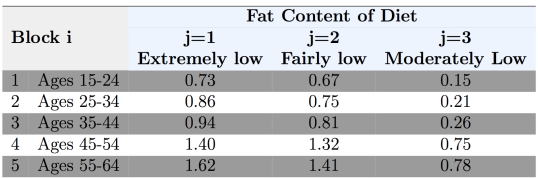
\includegraphics{1.png}
\caption{}
\end{figure}

    \subsubsection*{(a)}\label{a}

Why do you think that age of subject was used as a blocking variable? \\

    Because age is a confounding factor and the total fat level might be
varied depending on ages, so age should be used as a blocking variable.

    \subsubsection*{(b)}\label{b}

Obtain the residuals for randomized block model
\(Y_{ij} = \mu + \tau_{i} + \beta_j + \epsilon_{ij}\) and plot them
against the fitted values. Also prepare a normal probability plot of the
residuals. What are your findings?

    \begin{Verbatim}[commandchars=\\\{\}]
{\color{incolor}In [{\color{incolor}18}]:} fat \PY{o}{=} \PY{k+kt}{c}\PY{p}{(}\PY{l+m}{0.73}\PY{p}{,}\PY{l+m}{0.67}\PY{p}{,}\PY{l+m}{0.15}\PY{p}{,}\PY{l+m}{0.86}\PY{p}{,}\PY{l+m}{0.75}\PY{p}{,}\PY{l+m}{0.21}\PY{p}{,}\PY{l+m}{0.94}\PY{p}{,}\PY{l+m}{0.81}\PY{p}{,}\PY{l+m}{0.26}\PY{p}{,}\PY{l+m}{1.40}\PY{p}{,}\PY{l+m}{1.32}\PY{p}{,}\PY{l+m}{0.75}\PY{p}{,}\PY{l+m}{1.62}\PY{p}{,}\PY{l+m}{1.41}\PY{p}{,}\PY{l+m}{0.78}\PY{p}{)}
         diet \PY{o}{=} \PY{k+kp}{rep}\PY{p}{(}\PY{k+kt}{c}\PY{p}{(}\PY{l+s}{\PYZdq{}}\PY{l+s}{j1\PYZdq{}}\PY{p}{,} \PY{l+s}{\PYZdq{}}\PY{l+s}{j2\PYZdq{}}\PY{p}{,} \PY{l+s}{\PYZdq{}}\PY{l+s}{j3\PYZdq{}}\PY{p}{)}\PY{p}{,} \PY{l+m}{5}\PY{p}{)}
         age \PY{o}{=} \PY{k+kt}{c}\PY{p}{(}\PY{k+kp}{rep}\PY{p}{(}\PY{l+s}{\PYZdq{}}\PY{l+s}{15\PYZhy{}24\PYZdq{}}\PY{p}{,} \PY{l+m}{3}\PY{p}{)}\PY{p}{,} \PY{k+kp}{rep}\PY{p}{(}\PY{l+s}{\PYZdq{}}\PY{l+s}{25\PYZhy{}34\PYZdq{}}\PY{p}{,} \PY{l+m}{3}\PY{p}{)}\PY{p}{,} \PY{k+kp}{rep}\PY{p}{(}\PY{l+s}{\PYZdq{}}\PY{l+s}{35\PYZhy{}44\PYZdq{}}\PY{p}{,} \PY{l+m}{3}\PY{p}{)}\PY{p}{,} \PY{k+kp}{rep}\PY{p}{(}\PY{l+s}{\PYZdq{}}\PY{l+s}{45\PYZhy{}54\PYZdq{}}\PY{p}{,} \PY{l+m}{3}\PY{p}{)}\PY{p}{,}
          \PY{k+kp}{rep}\PY{p}{(}\PY{l+s}{\PYZdq{}}\PY{l+s}{55\PYZhy{}64\PYZdq{}}\PY{p}{,} \PY{l+m}{3}\PY{p}{)}\PY{p}{)}
         df \PY{o}{=} \PY{k+kt}{data.frame}\PY{p}{(}fat\PY{p}{,} diet\PY{p}{,} age\PY{p}{)}
         df
\end{Verbatim}

    \begin{tabular}{r|lll}
 fat & diet & age\\
\hline
	 0.73  & j1    & 15-24\\
	 0.67  & j2    & 15-24\\
	 0.15  & j3    & 15-24\\
	 0.86  & j1    & 25-34\\
	 0.75  & j2    & 25-34\\
	 0.21  & j3    & 25-34\\
	 0.94  & j1    & 35-44\\
	 0.81  & j2    & 35-44\\
	 0.26  & j3    & 35-44\\
	 1.40  & j1    & 45-54\\
	 1.32  & j2    & 45-54\\
	 0.75  & j3    & 45-54\\
	 1.62  & j1    & 55-64\\
	 1.41  & j2    & 55-64\\
	 0.78  & j3    & 55-64\\
\end{tabular}


    
    \begin{Verbatim}[commandchars=\\\{\}]
{\color{incolor}In [{\color{incolor}8}]:} fat.lm \PY{o}{=} lm\PY{p}{(}fat \PY{o}{\PYZti{}} diet\PY{o}{+}age\PY{p}{,} data\PY{o}{=}df\PY{p}{)} 
        fat.res \PY{o}{=} resid\PY{p}{(}fat.lm\PY{p}{)}
        diet\PYZus{}1\PYZus{}res \PY{o}{=} fat.res\PY{p}{[}\PY{k+kt}{c}\PY{p}{(}\PY{l+m}{1}\PY{p}{,} \PY{l+m}{4}\PY{p}{,} \PY{l+m}{7}\PY{p}{,} \PY{l+m}{10}\PY{p}{,} \PY{l+m}{13}\PY{p}{)}\PY{p}{]}
        diet\PYZus{}2\PYZus{}res \PY{o}{=} fat.res\PY{p}{[}\PY{k+kt}{c}\PY{p}{(}\PY{l+m}{2}\PY{p}{,} \PY{l+m}{5}\PY{p}{,} \PY{l+m}{8}\PY{p}{,} \PY{l+m}{11}\PY{p}{,} \PY{l+m}{14}\PY{p}{)}\PY{p}{]}
        diet\PYZus{}3\PYZus{}res \PY{o}{=} fat.res\PY{p}{[}\PY{k+kt}{c}\PY{p}{(}\PY{l+m}{3}\PY{p}{,} \PY{l+m}{6}\PY{p}{,} \PY{l+m}{9}\PY{p}{,} \PY{l+m}{12}\PY{p}{,} \PY{l+m}{15}\PY{p}{)}\PY{p}{]}
        diet\PYZus{}1\PYZus{}res
        diet\PYZus{}2\PYZus{}res
        diet\PYZus{}3\PYZus{}res
\end{Verbatim}

    \begin{itemize}
\item[1] -0.0526666666666666
\item[4] -0.0126666666666666
\item[7] 0.00399999999999987
\item[10] -0.0226666666666668
\item[13] 0.0840000000000001
\end{itemize}

\[\]
    
    \begin{itemize}
\item[2] 0.00533333333333322
\item[5] -0.00466666666666661
\item[8] -0.00799999999999996
\item[11] 0.0153333333333334
\item[14] -0.00800000000000009
\end{itemize}

\[\]
    
    \begin{itemize}
\item[3] 0.0473333333333334
\item[6] 0.0173333333333332
\item[9] 0.00400000000000009
\item[12] 0.00733333333333337
\item[15] -0.076
\end{itemize}

\[\]

    
    \begin{Verbatim}[commandchars=\\\{\}]
{\color{incolor}In [{\color{incolor}9}]:} par\PY{p}{(}mfrow\PY{o}{=}\PY{k+kt}{c}\PY{p}{(}\PY{l+m}{2}\PY{p}{,}\PY{l+m}{2}\PY{p}{)}\PY{p}{)}
        plot\PY{p}{(}aov\PY{p}{(}fat.lm\PY{p}{)}\PY{p}{)}
\end{Verbatim}

    \begin{center}
    \adjustimage{max size={0.9\linewidth}{0.9\paperheight}}{output_6_0.png}
    \end{center}
    { \hspace*{\fill} \\}
    
    \begin{itemize}
\item
  From the Residual vs. Fitted plot we can see that for each vertical
  line of points representing a different treatment, the spread on the
  points appear to be approximately equal, indicating that these 3
  treatments have the same variance. So the assumption of constant
  variance is not violated.
\item
  From the QQ-plot above we could conclude that since not all the points
  fall on the dotted line, thus the residuals are not normal, it also
  appears to be heavy tailed.
\end{itemize}

    \subsubsection*{(c)}\label{c}

\begin{enumerate}
\def\labelenumi{(\alph{enumi})}
\setcounter{enumi}{2}
\tightlist
\item
  Plot the response \(Y_{ij}\) by blocks (Present the lipid levels for
  each kind of diet by block). What does this plot suggest about the
  appropriateness of the no-interaction assumption here?
\end{enumerate}

    \begin{Verbatim}[commandchars=\\\{\}]
{\color{incolor}In [{\color{incolor}10}]:} \PY{k+kn}{library}\PY{p}{(}ggplot2\PY{p}{)}
         \PY{k+kn}{library}\PY{p}{(}reshape2\PY{p}{)}
         
         dataset \PY{o}{=} \PY{l+s}{\PYZdq{}}
         \PY{l+s}{diet 15\PYZus{}to\PYZus{}24   25\PYZus{}to\PYZus{}34  35\PYZus{}to\PYZus{}44   45\PYZus{}to\PYZus{}54   55\PYZus{}to\PYZus{}64  }
         \PY{l+s}{1   0.73    0.86    0.94    1.40    1.62   }
         \PY{l+s}{2   0.67    0.75    0.81    1.32    1.41    }
         \PY{l+s}{3   0.15    0.21    0.26    0.75    0.78\PYZdq{}}
         
         df \PY{o}{=} read.table\PY{p}{(}text\PY{o}{=}dataset\PY{p}{,} header \PY{o}{=} \PY{k+kc}{TRUE}\PY{p}{)}
         
         melted\PYZus{}data \PY{o}{=} melt\PY{p}{(}df\PY{p}{,} id.vars \PY{o}{=} \PY{l+s}{\PYZdq{}}\PY{l+s}{diet\PYZdq{}}\PY{p}{,}
                     variable.name\PY{o}{=}\PY{l+s}{\PYZdq{}}\PY{l+s}{age\PYZdq{}}\PY{p}{,} value.name\PY{o}{=}\PY{l+s}{\PYZdq{}}\PY{l+s}{fat\PYZdq{}}\PY{p}{)} 
         
         ggplot\PY{p}{(}melted\PYZus{}data\PY{p}{,} aes\PY{p}{(}x \PY{o}{=} diet\PY{p}{,} y \PY{o}{=} fat\PY{p}{,} color\PY{o}{=}age\PY{p}{)}\PY{p}{)} \PY{o}{+} geom\PYZus{}point\PY{p}{(}\PY{p}{)} \PY{o}{+} geom\PYZus{}line\PY{p}{(}\PY{p}{)} \PY{o}{+}
         	 xlab\PY{p}{(}\PY{l+s}{\PYZsq{}}\PY{l+s}{diet type\PYZsq{}}\PY{p}{)} \PY{o}{+} ylab\PY{p}{(}\PY{l+s}{\PYZsq{}}\PY{l+s}{lipid level\PYZsq{}}\PY{p}{)}
\end{Verbatim}

    
    
    \begin{center}
    \adjustimage{max size={0.9\linewidth}{0.9\paperheight}}{output_9_1.png}
    \end{center}
    { \hspace*{\fill} \\}
    
    The no-interaction assumption is appropriate here since all five lines
are approximately parallel.

    \subsection*{Q2}\label{q2}

\begin{enumerate}
\def\labelenumi{\arabic{enumi}.}
\setcounter{enumi}{1}
\tightlist
\item
  (40 points) (By hand) Refer to the Fat in diets problem. Assume that
  randomized block model is appropriate.
\end{enumerate}

    \subsubsection*{(a)}\label{a}

\begin{enumerate}
\def\labelenumi{(\alph{enumi})}
\tightlist
\item
  Obtain the analysis of variance table.
\end{enumerate}

    \[\bar y_{.j1} = 1.11\] \[\bar y_{.j2} = 0.992\] \[\bar y_{.j3} = 0.43\]

\[\bar y_{age1.} = 0.517\] \[\bar y_{age2.} = 0.607\]
\[\bar y_{age3.} = 0.67\] \[\bar y_{age4.} = 1.157\]
\[\bar y_{age5.} = 1.27\]

\[\bar y_{..} = 0.844\]

\[SST_{diet} =  5 \cdot (1.11-0.844)^2 + 5 \cdot(0.992-0.844)^2 + 5\cdot(0.43-0.844)^2=1.32028\]

\[SSBlock = 3 \cdot(0.517-0.844)^2 + 3 \cdot(0.607-0.844)^2 + 3 \cdot(0.67-0.844)^2 + 3 \cdot(1.157-0.844)^2 + 3 \cdot(1.27-0.844)^2\]
\[ = 1.41896\]

\[SSTOTAL = (0.73-0.844)^2+(0.67-0.844)^2+(0.15-0.844)^2+(0.86-0.844)^2+(0.75-0.844)^2\]
\[+(0.21-0.844)^2+(0.94-0.844)^2+(0.81-0.844)^2+(0.26-0.844)^2+(1.4-0.844)^2+(1.32-0.844)^2\]
\[+(0.75-0.844)^2+(1.62-0.844)^2+(1.41-0.844)^2+(0.78-0.844)^2 = 2.75856\]

\[SSE = SSTOTAL - SST - SSBlock = 2.75856 - 1.32028 - 1.41896 = 0.01932\]

\[MSB = \frac{SST}{3-1} = 0.660140\]

\[MSBlock = \frac{SSBlock}{5-1} = 0.354740\]

\[MSE = \frac{SST}{(3-1)(5-1)} = 0002415\]

\[F_{diet} = \frac{MSB}{MSE} = \frac{0.660140}{0.002415} = 273.3409\]

\[F_{block} =\frac{MSBlock}{MSE} = \frac{0.354740}{0.002415} = 146.8903\]

    \begin{Verbatim}[commandchars=\\\{\}]
{\color{incolor}In [{\color{incolor}19}]:} \PY{c+c1}{\PYZsh{} check my answer}
         \PY{k+kn}{library}\PY{p}{(}knitr\PY{p}{)}
         \PY{k+kn}{library}\PY{p}{(}lsmeans\PY{p}{)}
         aov.fat \PY{o}{=} aov\PY{p}{(}fat \PY{o}{\PYZti{}} diet\PY{o}{+}age\PY{p}{,} data\PY{o}{=}df\PY{p}{)}
         kable\PY{p}{(}anova\PY{p}{(}aov.fat\PY{p}{)}\PY{p}{,} format\PY{o}{=}\PY{l+s}{\PYZsq{}}\PY{l+s}{markdown\PYZsq{}}\PY{p}{)}
\end{Verbatim}

    
    \begin{verbatim}


|          | Df|  Sum Sq|  Mean Sq|  F value| Pr(>F)|
|:---------|--:|-------:|--------:|--------:|------:|
|diet      |  2| 1.32028| 0.660140| 273.3499|  0e+00|
|age       |  4| 1.41896| 0.354740| 146.8903|  2e-07|
|Residuals |  8| 0.01932| 0.002415|       NA|     NA|
    \end{verbatim}

    
    \subsubsection*{(b)}\label{b}

Test whether or not the mean reductions in lipid level differ for the
three diets; use α = 0.05. State the alternatives, decision rule, and
conclusion. What is the P-value of the test?

    \textbf{Null Hypothesis:}

\[H_0: \tau_1 = \tau_2 = \tau_3 = 0\]

\[H_a: \text{ there exists at least one } \tau_i \text{ that's not equal to } 0\]

And from the calculation in question part (a), we get the p-value of
diet as:

    \begin{Verbatim}[commandchars=\\\{\}]
{\color{incolor}In [{\color{incolor}20}]:} p\PYZus{}value \PY{o}{=} \PY{l+m}{0e+00}
         p\PYZus{}value \PY{o}{\PYZlt{}} \PY{l+m}{0.05}
\end{Verbatim}

    TRUE

    
    Since p-value \(<0.05\), thus we are confident enough to reject the null
hypothesis that \(H_0: \tau_1 = \tau_2 = \tau_3 = 0\), indicating that
the mean reductions in lipid level differ for the three diets.

    \subsubsection*{(c)}\label{c}

\begin{enumerate}
\def\labelenumi{(\alph{enumi})}
\setcounter{enumi}{2}
\tightlist
\item
  If there is significant difference in lipid level, how do they differ?
\end{enumerate}

    \begin{Verbatim}[commandchars=\\\{\}]
{\color{incolor}In [{\color{incolor}21}]:} TukeyHSD\PY{p}{(}aov\PY{p}{(}fat.lm\PY{p}{)}\PY{p}{,}\PY{l+s}{\PYZdq{}}\PY{l+s}{diet\PYZdq{}}\PY{p}{)}
\end{Verbatim}

    
    \begin{verbatim}
  Tukey multiple comparisons of means
    95% family-wise confidence level

Fit: aov(formula = fat.lm)

$diet
        diff        lwr         upr     p adj
j2-j1 -0.118 -0.2068109 -0.02918909 0.0129653
j3-j1 -0.680 -0.7688109 -0.59118909 0.0000000
j3-j2 -0.562 -0.6508109 -0.47318909 0.0000002

    \end{verbatim}

    
    \subsection*{Q3}\label{q3}

\begin{enumerate}
\def\labelenumi{\arabic{enumi}.}
\setcounter{enumi}{2}
\tightlist
\item
  (45 points) (ANCOVA) A manufacturer of felt-tip markers investigated
  by an experiment whether a proposed new display, featuring a picture
  of a physician, is more effective in drugstores than the present
  counter display, featuring a picture of an athlete and designed to be
  located in the stationary area. Fifteen drugstores of similar
  characteristics were chosen for the study. They were assigned at
  random in equal numbers to one of the following treatments: (1)
  present counter display in stationary area, (2) new display in
  stationary area, (3) new display in checkout area. Sales with the
  present display (X it ) were recorded in all 15 stores for a three
  week period. Then the new display was set up in the 10 stores
  receiving it, and sales for the next three week period (Y it ) were
  recorded in all 15 stores. The data on sales (in dollars) follow.
\end{enumerate}

\begin{figure}[H]
\centering
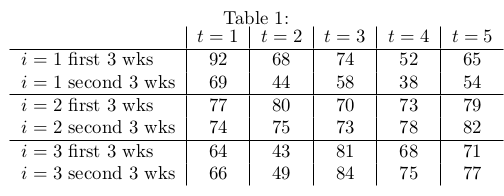
\includegraphics{2.png}
\caption{}
\end{figure}

The analyst wishes to analyze the effects of the three different display
treatments by means of covariance analysis.

    \subsubsection*{(a)}\label{a}

\begin{enumerate}
\def\labelenumi{(\alph{enumi})}
\tightlist
\item
  Obtain the residuals for covariance model
  \(Y_{it} = \mu + \tau_{i}+ \gamma(X_{it} - \bar X_{..} ) + \epsilon_{it}\).
\end{enumerate}

    \begin{Verbatim}[commandchars=\\\{\}]
{\color{incolor}In [{\color{incolor}22}]:} x \PY{o}{=}  \PY{k+kt}{c}\PY{p}{(}\PY{l+m}{92}\PY{p}{,}\PY{l+m}{68}\PY{p}{,}\PY{l+m}{74}\PY{p}{,}\PY{l+m}{52}\PY{p}{,}\PY{l+m}{65}\PY{p}{,}
                \PY{l+m}{77}\PY{p}{,}\PY{l+m}{80}\PY{p}{,}\PY{l+m}{70}\PY{p}{,}\PY{l+m}{73}\PY{p}{,}\PY{l+m}{79}\PY{p}{,}
                \PY{l+m}{64}\PY{p}{,}\PY{l+m}{43}\PY{p}{,}\PY{l+m}{81}\PY{p}{,}\PY{l+m}{68}\PY{p}{,}\PY{l+m}{71}\PY{p}{)}
         sales \PY{o}{=} \PY{k+kt}{c}\PY{p}{(}\PY{l+m}{69}\PY{p}{,}\PY{l+m}{44}\PY{p}{,}\PY{l+m}{58}\PY{p}{,}\PY{l+m}{38}\PY{p}{,}\PY{l+m}{54}\PY{p}{,}
                   \PY{l+m}{74}\PY{p}{,}\PY{l+m}{75}\PY{p}{,}\PY{l+m}{73}\PY{p}{,}\PY{l+m}{78}\PY{p}{,}\PY{l+m}{82}\PY{p}{,}
                   \PY{l+m}{66}\PY{p}{,}\PY{l+m}{49}\PY{p}{,}\PY{l+m}{84}\PY{p}{,}\PY{l+m}{75}\PY{p}{,}\PY{l+m}{77}\PY{p}{)}
         time \PY{o}{=} \PY{k+kp}{rep}\PY{p}{(}\PY{k+kt}{c}\PY{p}{(}\PY{l+s}{\PYZdq{}}\PY{l+s}{t1\PYZdq{}}\PY{p}{,} \PY{l+s}{\PYZdq{}}\PY{l+s}{t2\PYZdq{}}\PY{p}{,} \PY{l+s}{\PYZdq{}}\PY{l+s}{t3\PYZdq{}}\PY{p}{,} \PY{l+s}{\PYZdq{}}\PY{l+s}{t4\PYZdq{}}\PY{p}{,} \PY{l+s}{\PYZdq{}}\PY{l+s}{t5\PYZdq{}}\PY{p}{)}\PY{p}{,} \PY{l+m}{3}\PY{p}{)}
         display \PY{o}{=} \PY{k+kt}{c}\PY{p}{(}\PY{k+kp}{rep}\PY{p}{(}\PY{l+s}{\PYZdq{}}\PY{l+s}{i1\PYZdq{}}\PY{p}{,} \PY{l+m}{5}\PY{p}{)}\PY{p}{,} \PY{k+kp}{rep}\PY{p}{(}\PY{l+s}{\PYZdq{}}\PY{l+s}{i2\PYZdq{}}\PY{p}{,} \PY{l+m}{5}\PY{p}{)}\PY{p}{,} \PY{k+kp}{rep}\PY{p}{(}\PY{l+s}{\PYZdq{}}\PY{l+s}{i3\PYZdq{}}\PY{p}{,} \PY{l+m}{5}\PY{p}{)}\PY{p}{)}
         df \PY{o}{=} \PY{k+kt}{data.frame}\PY{p}{(}x\PY{p}{,} sales\PY{p}{,} display\PY{p}{,} time\PY{p}{)}
         df
\end{Verbatim}

    \begin{tabular}{r|llll}
 x & sales & display & time\\
\hline
	 92 & 69 & i1 & t1\\
	 68 & 44 & i1 & t2\\
	 74 & 58 & i1 & t3\\
	 52 & 38 & i1 & t4\\
	 65 & 54 & i1 & t5\\
	 77 & 74 & i2 & t1\\
	 80 & 75 & i2 & t2\\
	 70 & 73 & i2 & t3\\
	 73 & 78 & i2 & t4\\
	 79 & 82 & i2 & t5\\
	 64 & 66 & i3 & t1\\
	 43 & 49 & i3 & t2\\
	 81 & 84 & i3 & t3\\
	 68 & 75 & i3 & t4\\
	 71 & 77 & i3 & t5\\
\end{tabular}


    
    \begin{Verbatim}[commandchars=\\\{\}]
{\color{incolor}In [{\color{incolor}23}]:} sales.lm \PY{o}{=} lm\PY{p}{(}sales \PY{o}{\PYZti{}} \PY{k+kp}{I}\PY{p}{(}x\PY{o}{\PYZhy{}}\PY{k+kp}{mean}\PY{p}{(}x\PY{p}{)}\PY{p}{)} \PY{o}{+} display\PY{p}{,} data\PY{o}{=}df\PY{p}{)} 
         sales.res \PY{o}{=} resid\PY{p}{(}sales.lm\PY{p}{)}
         display\PYZus{}1\PYZus{}res \PY{o}{=} sales.res\PY{p}{[}\PY{l+m}{1}\PY{o}{:}\PY{l+m}{5}\PY{p}{]}
         display\PYZus{}2\PYZus{}res \PY{o}{=} sales.res\PY{p}{[}\PY{l+m}{6}\PY{o}{:}\PY{l+m}{10}\PY{p}{]}
         display\PYZus{}3\PYZus{}res \PY{o}{=} sales.res\PY{p}{[}\PY{l+m}{11}\PY{o}{:}\PY{l+m}{15}\PY{p}{]}
         display\PYZus{}1\PYZus{}res
         display\PYZus{}2\PYZus{}res
         display\PYZus{}3\PYZus{}res
\end{Verbatim}

    \begin{itemize}
\item[1] -1.79728464419479
\item[2] -6.7635767790262
\item[3] 2.22799625468167
\item[4] 0.592228464419472
\item[5] 5.74063670411986
\end{itemize}

\[\]
    
    \begin{itemize}
\item[6] -3.40168539325843
\item[7] -4.90589887640449
\item[8] 1.44147940074906
\item[9] 3.93726591760299
\item[10] 2.92883895131086
\end{itemize}

\[\]
    
    \begin{itemize}
\item[11] -3.0313670411985
\item[12] -2.50187265917605
\item[13] 0.778089887640463
\item[14] 2.62968164794008
\item[15] 2.12546816479401
\end{itemize}


    
    \subsubsection*{(b)}\label{b}

\begin{enumerate}
\def\labelenumi{(\alph{enumi})}
\setcounter{enumi}{1}
\tightlist
\item
  For each treatment, plot the residuals against the fitted values. Also
  prepare a normal probability plot of the residuals.
\end{enumerate}

    \begin{Verbatim}[commandchars=\\\{\}]
{\color{incolor}In [{\color{incolor}24}]:} par\PY{p}{(}mfrow\PY{o}{=}\PY{k+kt}{c}\PY{p}{(}\PY{l+m}{2}\PY{p}{,}\PY{l+m}{2}\PY{p}{)}\PY{p}{)}
         plot\PY{p}{(}aov\PY{p}{(}sales.lm\PY{p}{)}\PY{p}{)}
\end{Verbatim}

    \begin{center}
    \adjustimage{max size={0.9\linewidth}{0.9\paperheight}}{output_26_0.png}
    \end{center}
    { \hspace*{\fill} \\}
    
    \begin{itemize}
\item
  From the Residual vs. Fitted plot we can see that for each vertical
  line of points representing a different treatment, the spread on the
  points appear to be approximately equal, indicating that these 3
  treatments have the same variance. So the assumption of constant
  variance is not violated.
\item
  From the QQ-plot above we could conclude that since almost all the
  points fall on the dotted line, thus the residuals are normal.
\end{itemize}

    \subsubsection*{(c)}\label{c}

Assume ANOVA with equal slope models, i.e.,
\(Y_{it} = \mu + \tau_i + \gamma(X_{it}- \bar X_{..} ) + \epsilon_{it}\).
Test for whether the slope is significant. Conduct the test using
\(\alpha\) = 0.05. State the alternatives, decision rule, and
conclusion. What is the P-value of the test?

\[\]
    Null Hypothesis:

\[H_0: \gamma = 0 \]

\noindent Alternative Hypothesis:

\[H_a: \gamma \neq 0 \]

    \begin{Verbatim}[commandchars=\\\{\}]
{\color{incolor}In [{\color{incolor}25}]:} aov.sales \PY{o}{=} aov\PY{p}{(}sales \PY{o}{\PYZti{}} \PY{k+kp}{I}\PY{p}{(}x\PY{o}{\PYZhy{}}\PY{k+kp}{mean}\PY{p}{(}x\PY{p}{)}\PY{p}{)}\PY{o}{+}display\PY{p}{)}
         kable\PY{p}{(}anova\PY{p}{(}aov.sales\PY{p}{)}\PY{p}{,} format\PY{o}{=}\PY{l+s}{\PYZsq{}}\PY{l+s}{markdown\PYZsq{}}\PY{p}{)}
\end{Verbatim}

    
    \begin{verbatim}


|               | Df|   Sum Sq|    Mean Sq|  F value|  Pr(>F)|
|:--------------|--:|--------:|----------:|--------:|-------:|
|I(x - mean(x)) |  1| 1317.789| 1317.78912| 82.11456| 2.0e-06|
|display        |  2| 1397.281|  698.64046| 43.53394| 5.9e-06|
|Residuals      | 11|  176.530|   16.04818|       NA|      NA|
    \end{verbatim}

    
    Since p value is smaller than \(\alpha=0.05\), thus we are confident
enough to reject the null hypothesis and reach the conclusion that the
slope is significant

    \subsubsection*{(d)}\label{d}

\begin{enumerate}
\def\labelenumi{(\alph{enumi})}
\setcounter{enumi}{3}
\tightlist
\item
  Fit the full and reduced regression models and test for treatment
  effects: use \(\alpha = 0.05\). State the alternatives, decision rule,
  and conclusion. What is the P-value of the test?
\end{enumerate}

    \textbf{Full Model:}

\[Y_{it} = \mu + \tau_{i} I_{it}  + \gamma x_{it} + \beta_i I_{it} x_{it}+ \epsilon_{it}\]

Null hypothesis:

\[H_0 : \beta_1 = \beta_2 = \beta_3 = 0\]

Alternative Hypothesis:

\[H a : \text{ not all } \beta_1, \beta_2 \text{ and } \beta_3 \text{ equal to zero}\]

    \begin{Verbatim}[commandchars=\\\{\}]
{\color{incolor}In [{\color{incolor}26}]:} aov.full \PY{o}{=} aov\PY{p}{(}sales \PY{o}{\PYZti{}} \PY{k+kp}{I}\PY{p}{(}x\PY{o}{\PYZhy{}}\PY{k+kp}{mean}\PY{p}{(}x\PY{p}{)}\PY{p}{)}\PY{o}{+}display\PY{o}{+}\PY{k+kp}{I}\PY{p}{(}x\PY{o}{\PYZhy{}}\PY{k+kp}{mean}\PY{p}{(}x\PY{p}{)}\PY{p}{)}\PY{o}{*}display\PY{p}{)}
         kable\PY{p}{(}anova\PY{p}{(}aov.full\PY{p}{)}\PY{p}{,} format\PY{o}{=}\PY{l+s}{\PYZsq{}}\PY{l+s}{markdown\PYZsq{}}\PY{p}{)}
\end{Verbatim}

    
    \begin{verbatim}


|                       | Df|     Sum Sq|    Mean Sq|    F value|    Pr(>F)|
|:----------------------|--:|----------:|----------:|----------:|---------:|
|I(x - mean(x))         |  1| 1317.78912| 1317.78912| 81.6807634| 0.0000083|
|display                |  2| 1397.28092|  698.64046| 43.3039592| 0.0000241|
|I(x - mean(x)):display |  2|   31.32929|   15.66464|  0.9709444| 0.4151222|
|Residuals              |  9|  145.20068|   16.13341|         NA|        NA|
    \end{verbatim}

    
    Since p value of I(x - mean(x)):display is larger than \(\alpha=0.05\),
thus we are not confident enough to reject the null hypothesis,
indicating the fact that \(\beta_1 = \beta_2 = \beta_3 = 0\).

    \textbf{Reduced Model:}

\[Y_{it} = \mu + \gamma x_{it} + \epsilon_{it}\]

Null hypothesis:

\[H_0 : \gamma = 0\]

Alternative Hypothesis:

\[H a : \gamma \neq 0\]

    \begin{Verbatim}[commandchars=\\\{\}]
{\color{incolor}In [{\color{incolor}27}]:} aov.reduced \PY{o}{=} aov\PY{p}{(}sales \PY{o}{\PYZti{}} \PY{k+kp}{I}\PY{p}{(}x\PY{o}{\PYZhy{}}\PY{k+kp}{mean}\PY{p}{(}x\PY{p}{)}\PY{p}{)}\PY{p}{)}
         kable\PY{p}{(}anova\PY{p}{(}aov.reduced\PY{p}{)}\PY{p}{,} format\PY{o}{=}\PY{l+s}{\PYZsq{}}\PY{l+s}{markdown\PYZsq{}}\PY{p}{)}
\end{Verbatim}

    
    \begin{verbatim}


|               | Df|   Sum Sq|   Mean Sq|  F value|    Pr(>F)|
|:--------------|--:|--------:|---------:|--------:|---------:|
|I(x - mean(x)) |  1| 1317.789| 1317.7891| 10.88521| 0.0057558|
|Residuals      | 13| 1573.811|  121.0624|       NA|        NA|
    \end{verbatim}

    
    Since p value of I(x - mean(x)) is smaller than \(\alpha=0.05\), thus we
are confident enough to reject the null hypothesis, indicating the fact
that \(\gamma \neq 0\).


    % Add a bibliography block to the postdoc
    
    
    
    \end{document}
